\section{Teoria}

\subsection{Lineaarialgebra}
Vektoriavaruuden $\mathbb{R}^m$ aliavaruuden $\mathbb{V}$ virittävät keskenään lineaarisesti riippumattomat vektorit $\{\mathbf{a_1,...,a_n}\}$, jota merkitään $\text{span}(\mathbf{a_1,...,a_n})$. Tällöin vektorit $(\mathbf{a_1,...,a_n})$ muodostavat aliavaruuden $\mathbb{V}$ kannan. 

Olkoon matriisi $\mathbf{A}\in \mathbb{R}^{m\times n}$, jonka rivien lukumäärä on $\mathit{m}$ ja sarakkeiden $\mathit{n}$. Matriisin \textbf{A} virittävät sen lineaarisesti riippumattomat sarakevektorit eli $\text{span}(\mathbf{A}) = \text{span}(\mathbf{A(:,1),...,A(:,n)})$.

Matriisin \textbf{A} aste eli $\text{rank}(\textbf{A})$ kuvaa matriisin lineaarisesti riippumattomien sarake- tai rivivektoreiden lukumäärää. Matriisi \textbf{A} on kääntyvä eli sillä on käänteismatriisi $\mathbf{A}^{-1}$, jos matriisin aste on yhtä kuin sen rivien tai sarakkeiden määrä eli $\text{rank}(\textbf{A})=m=n$.



Singulaariarvohajotelman avulla matriisi voidaan esittää sen ominaisarvojen ja ortonormaalien matriisien avulla

\begin{equation}
    \mathbf{A = UDV^T,}
\end{equation}
jossa matriisin $\mathbf{A}$ ominaisarvot ovat matriisin $\mathbf{D}$ diagonaalilla. 

%pseudoinverse
Pseudokäänteismatriisi $\mathbf{A^{\dagger}}$ on yleistys matriisin käänteismatriisille. Tämä joudutaan muodostamaan silloin, kun matriisi $\mathbf{A}$ ei ole kääntyvä. Pseudokäänteismatriisi saadaan muodostettua singulaariarvohajotelman avulla
\begin{equation}
    \mathbf{A^{\dagger} = VD^{\dagger}U^T}
\end{equation}

%projektio
Projektio aliavaruuteen $\text{span}(\mathbf{A})$ saadaan kaavalla
\begin{equation}
    \mathbf{\Pi_{span(A)} = AA^{\dagger}}
\end{equation}
ja tämän ortogonaaliseen aliavaruuteen saadaan
\begin{equation}
    \mathbf{\Pi_{span(A^{\bot})}=I-AA^{\dagger}}
\end{equation}
\begin{figure}[ht]
    \centering
    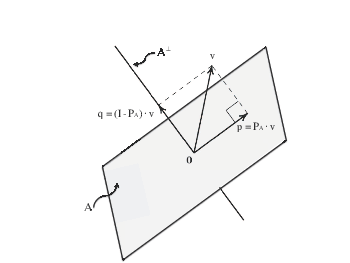
\includegraphics{ortoprojektio.png}.
    \caption{Ortoprojektio}
\end{figure}

\clearpage
\subsection{MUSIC}
MUSIC-algoritmi (Multiple Signal Classification) on \cite{Schmidt1986MultipleEstimation} kehittämä lähteenpaikannusmenetelmä, joka perustuu mittausdatan jakamiseen keskenään ortogonaalisiin signaali- ja kohina-aliavaruuksiin, jonka jälkeen tarkistetaan potentiaalisen lähteen topografian kuuluminen signaaliavaruuteen \citep{Mosher1999SourceMUSIC}. Algoritmissa lähteet kuvataan sähköisinä dipoleina ja se vaatii päämalliin tehdyn forward fieldin.

Tässä kerron ensin tavallisesta MUSIC-algoritmista, johon MUSIC-algoritmin muut versiot perustuvat. Tämän jälkeen kerron MUSIC-algoritmin iteratiivista versioista, RAP- sekä TRAP-MUSIC-algoritmeista.

Olkoon mittauksista saatu data kerättynä matriisiin $\mathbf{Y}\in \mathbb{R}^{m\times N}$, jossa $\mathit{m}$ on mittausanturien määrä ja $\mathit{N}$ mittausten lukumäärä. Matriisilla $\mathbf{Y}$ on muoto

\begin{equation}
    \mathbf{Y=AS+\epsilon},
\end{equation}
jossa $\mathbf{A}$ on sekoitusmatriisi, $\mathbf{S}$ ajankulkumatriisi ja $\mathbf{\epsilon}$ mittauskohinaa. Olkoon lähteellä paikassa $\mathbf{p}_j$ suuntaus $\mathbf{\eta}_j$. Tällöin lähteen topografia on $\mathbf{l}_j=\mathbf{l(p}_j,\mathbf{\eta}_j)$. Sekoitusmatriisi $\mathbf{A}$ sisältää lähteiden topografiat $\mathbf{\{l_1,...,l_n\}}$.

Data-avaruus $\text{span}(\mathbf{Y})$ jaetaan keskenään ortogonaalisiin signaaliavaruuteen $\text{span}(\mathbf{A})$  ja kohina-avaruuteen $\text{span}(\mathbf{A^\bot})$  \citep{Mosher1999SourceMUSIC}. Ortogonaaliprojektio signaaliavaruuteen $\text{span}(\mathbf{A})$ voidaan approksimoida kaavalla

\begin{equation}
    \textbf{P}_{s}=\textbf{U}(:,1:n)\textbf{U}(:,1:n)^T
\end{equation}

\begin{equation}
    \mu(\mathbf{p}) = \frac{||\mathbf{P}_s\mathbf{l(p)}||^2}{||\mathbf{l(p)}||^2}    
\end{equation}


\subsection{RAP-MUSIC}
RAP-MUSIC on MUSIC-algoritmin iteratiivinen versio, jossa lähteet paikannetaan yksitellen ja löydetyn lähteen topografia projisoidaan pois \citep{Mosher1999SourceMUSIC}. 

\subsubsection{RAP-dilemma}
RAP-MUSICin paikannusfunktio saattaa löytää lähdepisteitä jo löydettyjen lähteiden läheltä. Tämä johtuu siitä, ettei algoritmi pysty poistamaan topografiaa löydettyjen dipolien lähettyviltä \citep{Makela2018TruncatedLocalization}. Tätä RAP-dilemmaa havaitaan varsinkin kohinattomalla ja valkoisen kohinan datalla. Tämän algoritmin virheen korjaamiseksi \cite{Makela2018TruncatedLocalization} kehittivät ratkaisun, joka nimettiin TRAP-MUSICiksi. 

\subsection{TRAP-MUSIC}
Truncated RAP-MUSIC (TRAP-MUSIC) on muuten samankaltainen rekursiivinen algoritmi kuin RAP-MUSIC, mutta TRAP-MUSICin paikannusfunktioon on tehty pieni muutos: kun uusi lähde on löydetty, tämä kohta projisoidaan pois signaaliavaruudesta ja jäljellä oleva signaaliavaruus typistetään vastaamaan jäljellä olevien lähteiden arvioitua määrää \citep{Makela2018TruncatedLocalization}.